% Source: Code/ML_overlay/ir_rgb_registration/paper/ml_overlay_report_materials/ir_rgb_registration_report/figures/fig_flownet_architectures.tex
\documentclass[tikz,border=10pt]{standalone}
\usepackage{tikz}
\usetikzlibrary{positioning,shapes.geometric,arrows.meta,calc}

\definecolor{Garnet}{RGB}{115,0,10}
\definecolor{Rose}{RGB}{204,46,64}
\definecolor{Atlantic}{RGB}{70,106,159}
\definecolor{Congaree}{RGB}{31,65,77}
\definecolor{Black90}{RGB}{54,54,54}
\definecolor{Black70}{RGB}{92,92,92}

\begin{document}
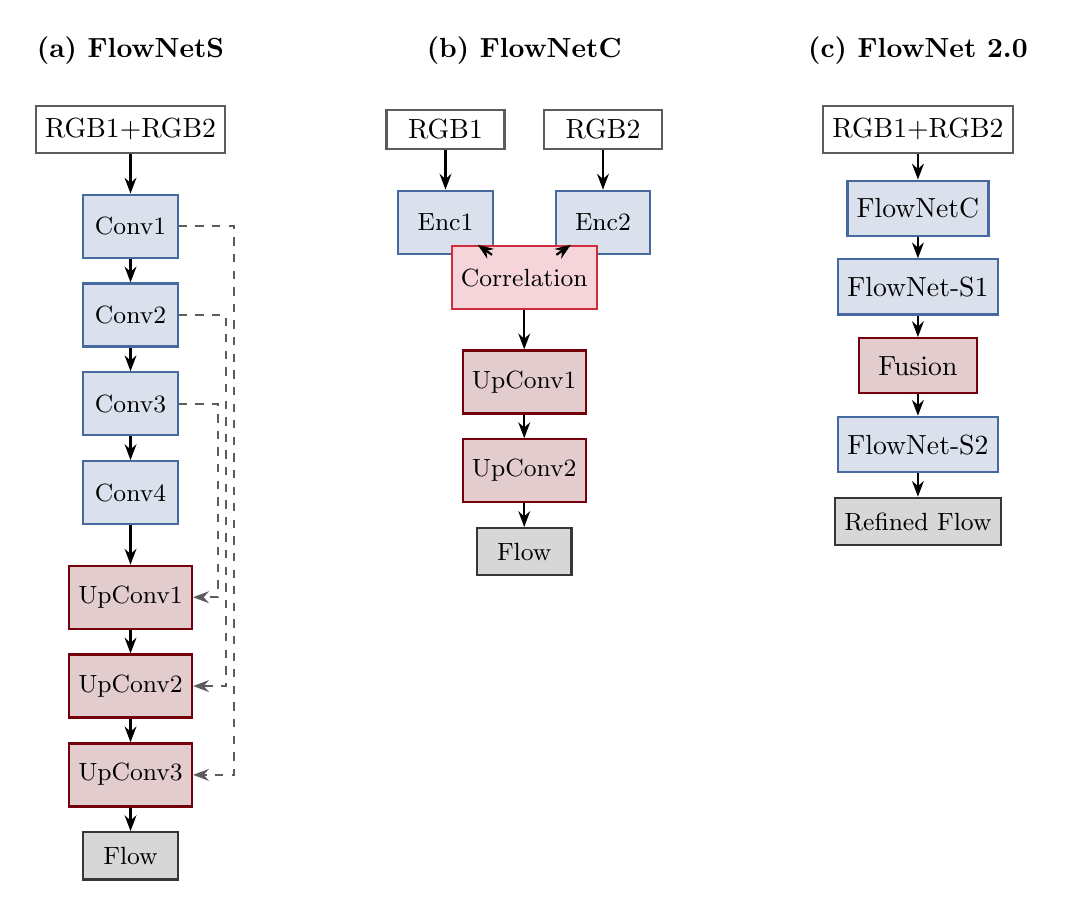
\begin{tikzpicture}[
    encoder/.style={rectangle,draw=Atlantic,fill=Atlantic!20,thick,minimum width=1.2cm,minimum height=0.8cm,font=\small},
    decoder/.style={rectangle,draw=Garnet,fill=Garnet!20,thick,minimum width=1.2cm,minimum height=0.8cm,font=\small},
    corr/.style={rectangle,draw=Rose,fill=Rose!20,thick,minimum width=1.2cm,minimum height=0.8cm,font=\small},
    flow/.style={rectangle,draw=Black90,fill=Black90!20,thick,minimum width=1.2cm,minimum height=0.6cm,font=\small},
    arrow/.style={-{Stealth[length=2mm]},thick}
]

% FlowNetS (left)
\node[font=\bfseries] at (0,5) {(a) FlowNetS};
\node[rectangle,draw=Black70,thick,minimum width=2cm,minimum height=0.6cm] (s-input) at (0,4) {RGB1+RGB2};
\node[encoder,below=0.5cm of s-input] (s-enc1) {Conv1};
\node[encoder,below=0.3cm of s-enc1] (s-enc2) {Conv2};
\node[encoder,below=0.3cm of s-enc2] (s-enc3) {Conv3};
\node[encoder,below=0.3cm of s-enc3] (s-enc4) {Conv4};
\node[decoder,below=0.5cm of s-enc4] (s-dec1) {UpConv1};
\node[decoder,below=0.3cm of s-dec1] (s-dec2) {UpConv2};
\node[decoder,below=0.3cm of s-dec2] (s-dec3) {UpConv3};
\node[flow,below=0.3cm of s-dec3] (s-flow) {Flow};

\draw[arrow] (s-input) -- (s-enc1);
\draw[arrow] (s-enc1) -- (s-enc2);
\draw[arrow] (s-enc2) -- (s-enc3);
\draw[arrow] (s-enc3) -- (s-enc4);
\draw[arrow] (s-enc4) -- (s-dec1);
\draw[arrow] (s-dec1) -- (s-dec2);
\draw[arrow] (s-dec2) -- (s-dec3);
\draw[arrow] (s-dec3) -- (s-flow);

% Skip connections
\draw[arrow,dashed,Black70] (s-enc3.east) -- ++(0.5,0) |- (s-dec1.east);
\draw[arrow,dashed,Black70] (s-enc2.east) -- ++(0.6,0) |- (s-dec2.east);
\draw[arrow,dashed,Black70] (s-enc1.east) -- ++(0.7,0) |- (s-dec3.east);

% FlowNetC (center)
\node[font=\bfseries] at (5,5) {(b) FlowNetC};
\node[rectangle,draw=Black70,thick,minimum width=1.5cm,minimum height=0.5cm] (c-in1) at (4,4) {RGB1};
\node[rectangle,draw=Black70,thick,minimum width=1.5cm,minimum height=0.5cm] (c-in2) at (6,4) {RGB2};
\node[encoder,below=0.5cm of c-in1] (c-enc1) {Enc1};
\node[encoder,below=0.5cm of c-in2] (c-enc2) {Enc2};
\node[corr,below=1.2cm of c-in1,xshift=1cm] (c-corr) {Correlation};
\node[decoder,below=0.5cm of c-corr] (c-dec1) {UpConv1};
\node[decoder,below=0.3cm of c-dec1] (c-dec2) {UpConv2};
\node[flow,below=0.3cm of c-dec2] (c-flow) {Flow};

\draw[arrow] (c-in1) -- (c-enc1);
\draw[arrow] (c-in2) -- (c-enc2);
\draw[arrow] (c-enc1) -- (c-corr);
\draw[arrow] (c-enc2) -- (c-corr);
\draw[arrow] (c-corr) -- (c-dec1);
\draw[arrow] (c-dec1) -- (c-dec2);
\draw[arrow] (c-dec2) -- (c-flow);

% FlowNet 2.0 (right)
\node[font=\bfseries] at (10,5) {(c) FlowNet 2.0};
\node[rectangle,draw=Black70,thick,minimum width=1.8cm,minimum height=0.6cm] (f2-input) at (10,4) {RGB1+RGB2};
\node[rectangle,draw=Atlantic,fill=Atlantic!20,thick,minimum width=1.5cm,minimum height=0.7cm] (f2-net1) at (10,3) {FlowNetC};
\node[rectangle,draw=Atlantic,fill=Atlantic!20,thick,minimum width=1.5cm,minimum height=0.7cm] (f2-net2) at (10,2) {FlowNet-S1};
\node[rectangle,draw=Garnet,fill=Garnet!20,thick,minimum width=1.5cm,minimum height=0.7cm] (f2-fuse) at (10,1) {Fusion};
\node[rectangle,draw=Atlantic,fill=Atlantic!20,thick,minimum width=1.5cm,minimum height=0.7cm] (f2-net3) at (10,0) {FlowNet-S2};
\node[flow,below=0.3cm of f2-net3] (f2-flow) {Refined Flow};

\draw[arrow] (f2-input) -- (f2-net1);
\draw[arrow] (f2-net1) -- (f2-net2);
\draw[arrow] (f2-net2) -- (f2-fuse);
\draw[arrow] (f2-fuse) -- (f2-net3);
\draw[arrow] (f2-net3) -- (f2-flow);

\end{tikzpicture}
\end{document}
